\section{Feedback}

If you could perfectly characterize a system, you could just keep sticking inputs into the system and know exactly what outputs would be produced. But this is impossible. Thus you need some way to monitor the output and adjust the input to react. These feedback systems can be modelled (and even implemented) as linear systems as well. Figure \ref{feedback_box} shows a representation of this.

\begin{figure}[h]
\centering
\includegraphics[scale=1.0]{feedback_box.png}
\caption{Linear System with Feedback}\label{feedback_box}
\end{figure}


The usual method of incorporating feedback is to simply subtract it from the primary input signal before sending the combined signal into the linear system. Figure \ref{feedback_box_2} shows this.

\begin{figure}[h]
\centering
\includegraphics[scale=1.0]{feedback_box_2.png}
\caption{Linear System with Feedback Showing Subtraction}\label{feedback_box_2}
\end{figure}